\chapter{Architettura e Design}
\label{ch:architectures}

\section{Design generale del software}

L'architettura del software è basata su micro-servizi autonomi e indipendenti tra loro e la loro comunicazione avviene tramite API REST.
Esiste un middleware che si occupa della gestione e dell'orchestrazione dei micro-servizi, facendo appunto da ponte collegando le varie diverse tencologie.

I microservizi che si sono scelti di sviluppare si occupano di varie aree legate alla natura del progetto e sono:
\begin{itemize}
    \item \textbf{ChatService}: si occupa della gestione delle chat tra utenti.
    \item \textbf{UserService}: si occupa della gestione degli utenti, quindi la loro registrazione, autenticazione e gestione dei dati personali.
    \item \textbf{BusinessLogic}: si occupa di mantenere al proprio interno tutte le regole proprie del gioco
    \item \textbf{Front-End}: si occupa di gestire l'interfaccia grafica e la comunicazione con il middleware.
    \item \textbf{Middleware}: si occupa della gestione delle comunicazioni tra i vari microservizi, e svolge la funzione di "motore di gioco".
\end{itemize}

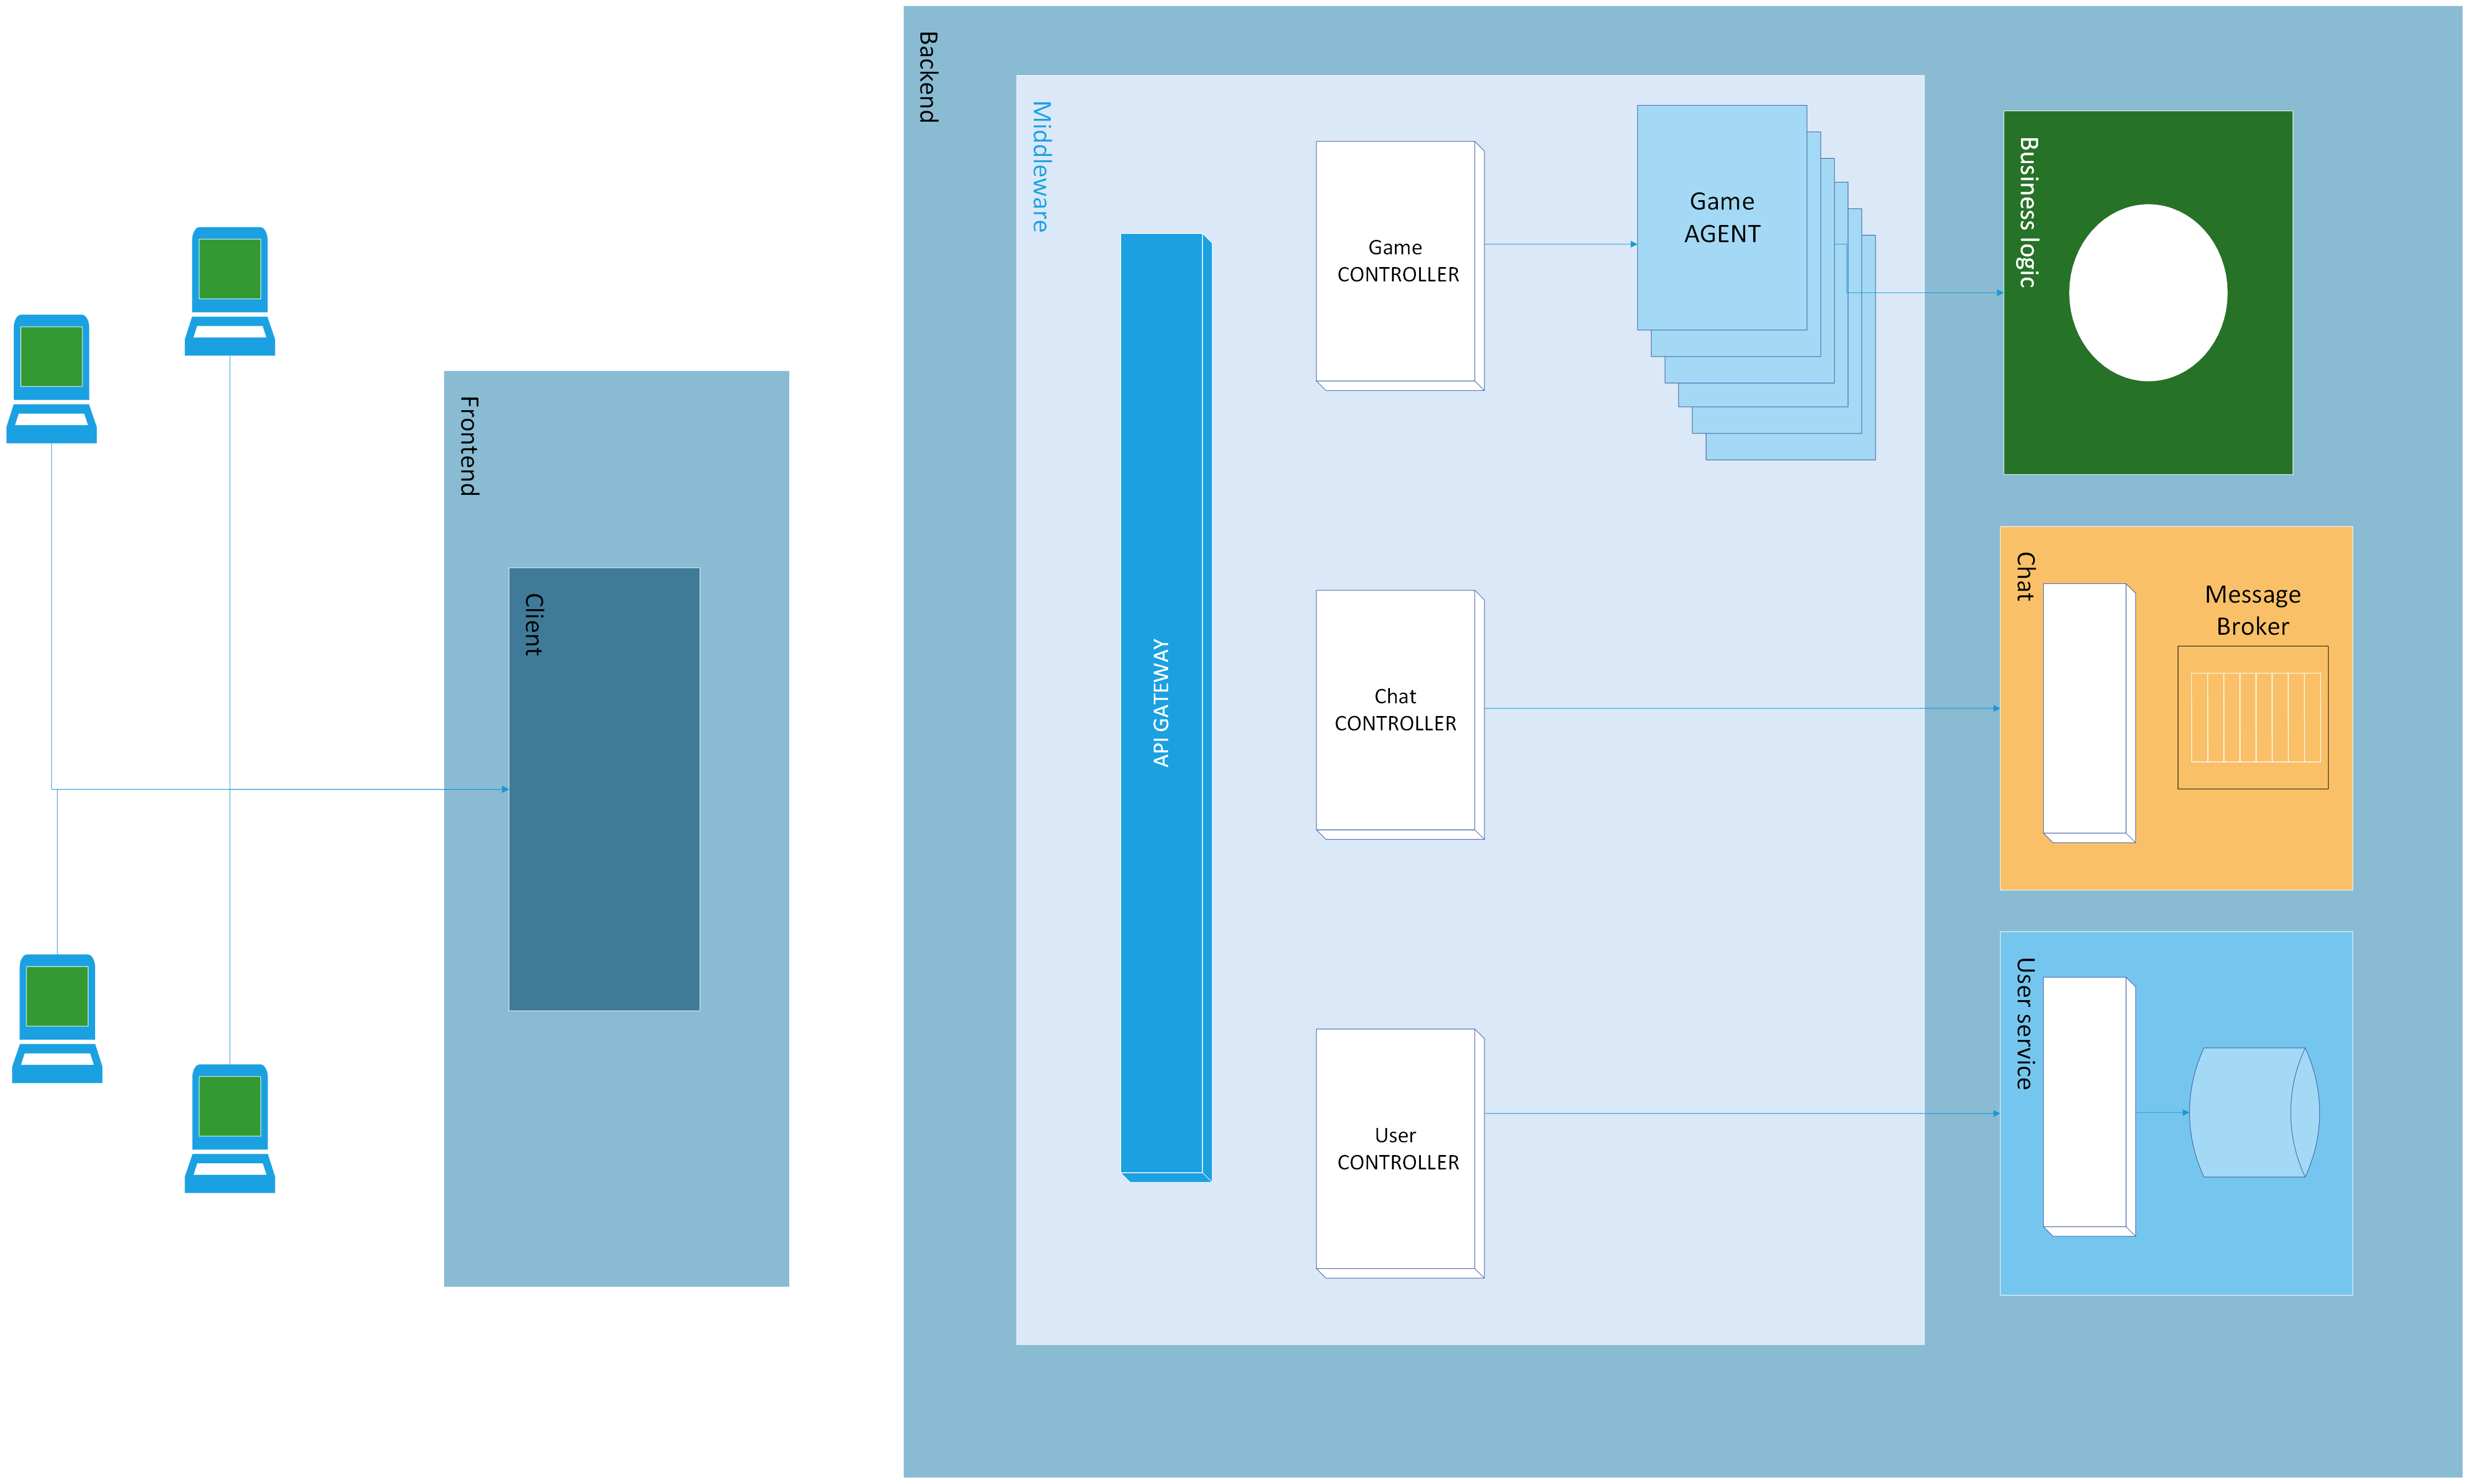
\includegraphics[width=12cm]{report/img/Architecture.png}\\[10.5cm]

\section{Micro-servizi e la loro architettura}

\subsection{Servizio per la Chat}

\begin{table}[h!]
    \centering
    \caption{Tabella descrittiva Chat Service}
    \label{tab:chat_serv_table}
    \begin{tabular}{ll}     
        \toprule                   
        Linguaggio & Java \\        
        Server & Vertx, Swagger \\
        Librerie & RabbitMQ(vertx) \\
        Architettura & Agenti vertx \\
        \bottomrule
    \end{tabular}
\end{table}

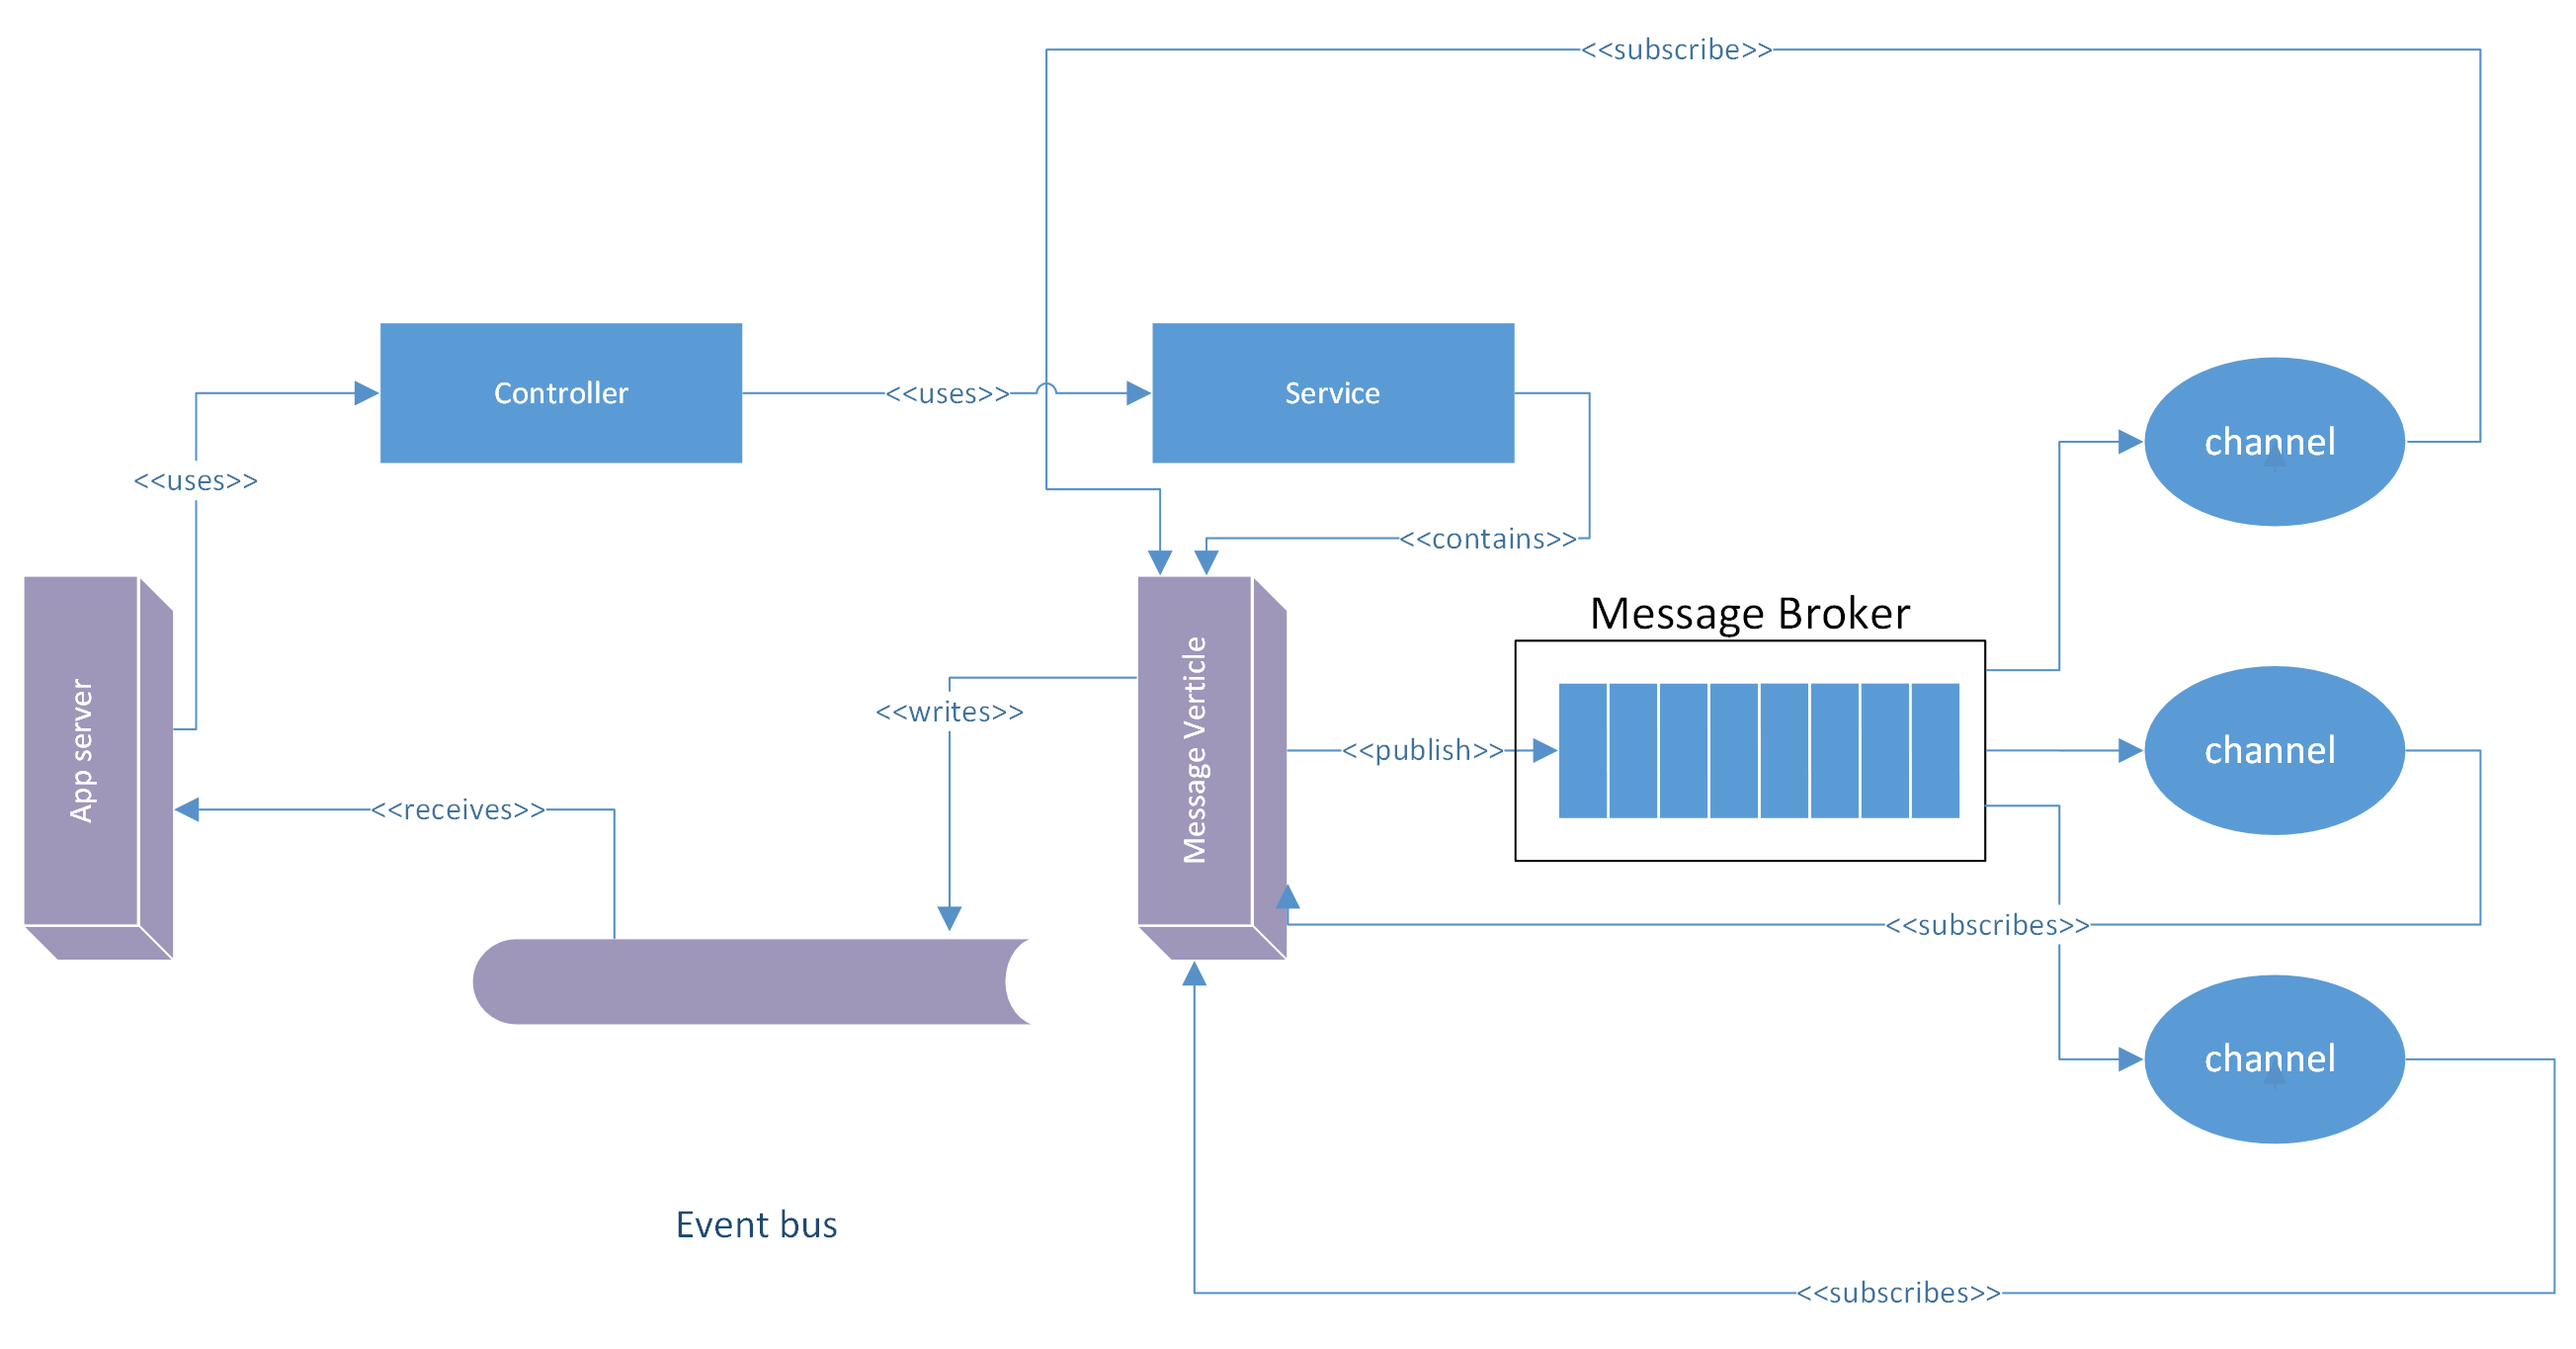
\includegraphics[width=15cm]{report/img/Architettura ChatService.png}\\[10.5cm]

\subsection{Servizio per Gestione Utenti}

\begin{table}[h!]
    \centering
    \caption{Tabella descrittiva User Service}
    \label{tab:user_serv_table}
    \begin{tabular}{ll}     
        \toprule                   
        Linguaggio & Node.JS/TypeScript \\        
        Framework & NestJS   \\                   
        Persistence & Mysql  \\
        Librerie & TypeORM   \\
        Architettura & Model-Controller-service  \\
        \bottomrule
    \end{tabular}
\end{table}


\subsection{Servizio Business Logic}

\begin{table}[h!]
    \centering
    \caption{Tabella descrittiva Business Logic}
    \label{tab:bl_serv_table}
    \begin{tabular}{ll}     
        \toprule                   
        Linguaggio & Node.JS/TypeScript \\        
        Framework & NestJS   \\                   
        Architettura & Model-Controller-service  \\
        \bottomrule
    \end{tabular}
\end{table}

\subsection{Servizio ponte tra i microservizi}


\begin{table}[h!]
    \centering
    \caption{Tabella descrittiva Middleware}
    \label{tab:middleware_serv_table}
    \begin{tabular}{ll}     
        \toprule                   
        Linguaggio & Java \\        
        Server & Vertx \\
        Librerie & RabbitMQ(vertx) \\
        Architettura & Multi-agent, motore di gioco \\
        \bottomrule
    \end{tabular}
\end{table}

\section{[DS/SPE] Perche' i microservizi?}

Ogni microservizio si occupa di gestire un singolo ambito di progetto, il che fa sì che si ottengano ottimi risultati  riguardo la qualità e l'affidabilità, la riutilizzabilità, la flessibilità e la scalabilità siano più
Tutti i componenti sono "loosely coupled", distribuiti in modo indipendente, e in ambiti reali gestiti da un piccolo team e altamente collaudabili e gestibili.
Tuttavia, non si tratta di una soluzione definitiva, ha anche degli svantaggi come ad esempio:
\begin{itemize}
    \item la complessità di gestione e la necessità di un'infrastruttura di rete molto complessa.
    \item un'ottima comunicazione di team.
    \item una discreta capacità di astrazione e progettazione di interfaccie di comunicazione che devono essere rispettate da tutti i microservizi.
    \item Non si ha la certezza che l'infrastruttura funzioni correttamente fino a quando tutti i servizi non cooperano tra loro.
\end{itemize}

\subsection{[SPE] Vantaggi}
- devops
- ci 

\subsection{[DS] Vantaggi}
- fault tolerance
- scalability
- docker